% ! TeX root = ...

\begin{frame}{Aggregate Computing \faPlus[l] Reinforcement Learning \href{https://github.com/cric96/scafi-with-reinforcement-learning}{\faLink}}
  \begin{backgroundblock} 
    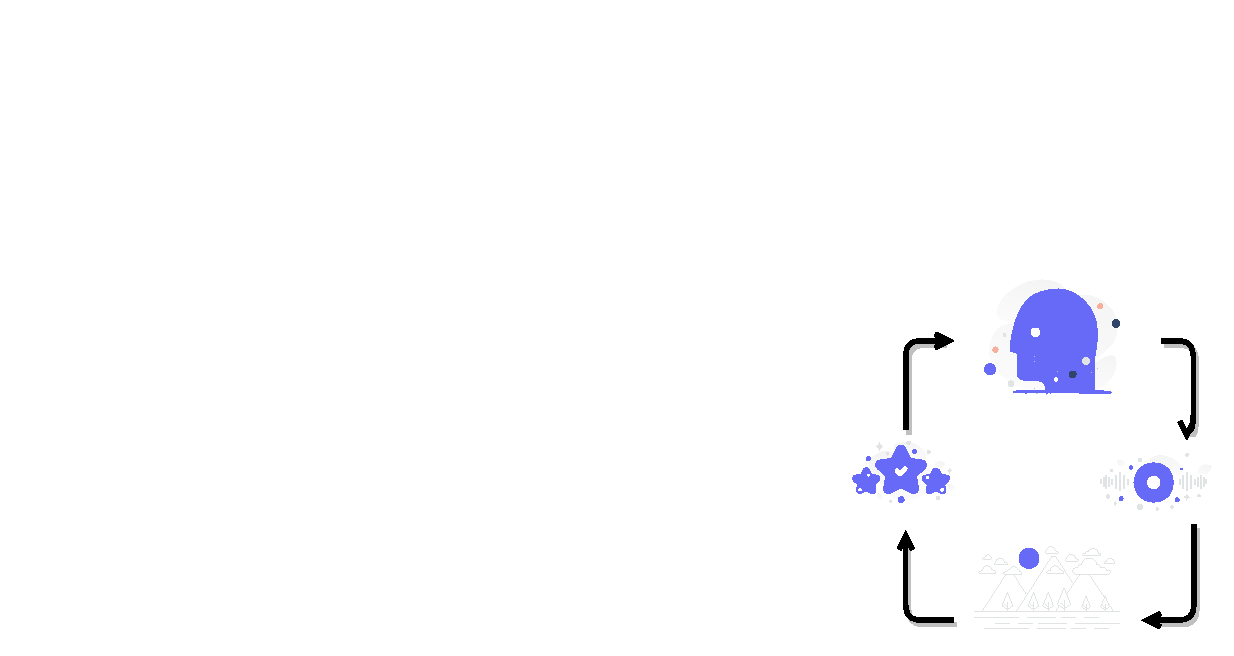
\includegraphics[width=\paperwidth]{img/rl-background.pdf} 
  \end{backgroundblock} 
  \begin{columns}[onlytextwidth]
    \begin{column}{0.7\textwidth}     
      \begin{card}[Most suitable match]
          \begin{itemize}
            \item <1->Typically used in CSAS
            \item <2->Designed to maximise long term rewards
            \item <3->Quite easy to express aggregate problems as reinforcement learning problems
          \end{itemize}
      \end{card}
  \end{column}
\end{columns}
  \pdfcomment{
    This combination seems to be one of the most suitable for several reasons: 
    i) in the literature, it seems the best way to integrate learning into CSAS 
    ii) it is designed to maximise the long term outcome, not just the best local response. 
    iii) even if the aggregate program seems to be a distributed regression, 
    it is quite easy to encode problems in terms of agent states and actions. 
  }
\end{frame}